\documentclass{article}
\usepackage{tikz}
\usepackage{fancyhdr}
\usepackage{geometry}
\usepackage[utf8]{inputenc}
\usepackage[hypertexnames=false, colorlinks=true, linkcolor=black]{hyperref}
\usepackage{listings}
\usepackage{xcolor}
\usepackage{tocloft}
\usepackage{palatino}  % Police

\usetikzlibrary{backgrounds, shapes.geometric, positioning}

\geometry{a4paper, left=15mm, right=15mm, top=30mm, bottom=30mm}

\pagestyle{fancy}
\fancyhf{}
\fancyhead[L]{Distance de Jaccard}
\fancyhead[R]{Projet Algorithmie 3}
\fancyhead[C]{De - backer Cuvelier Sébastien Llobregat Nicolas}
\fancyfoot[C]{\thepage}

\renewcommand{\contentsname}{Table des matières}

\setlength{\cftbeforesecskip}{20pt}
\setlength{\cftbeforesubsecskip}{10pt}
\setlength{\cftbeforesubsubsecskip}{5pt}

\newcommand{\fondpremierepage}{
  \begin{tikzpicture}[remember picture, overlay]
    \node[align=center, text width=0.8\textwidth, font=\huge\bfseries] at (current page.center) {
        Projet Algorithmie 3 La distance de Jaccard};
    \node[align=center, text width=0.8\textwidth, font=\large] at (current page.center) [yshift=-1.5cm] {
        De - backer Cuvelier Sébastien Llobregat Nicolas};
    \node[align=center, text width=0.8\textwidth, font=\normalsize] at (current page.center) [yshift=-2.5cm] {
        Version du 08 Avril 2025};
  \end{tikzpicture}
}

\lstdefinestyle{Cstyle}{
  language=C,
  basicstyle=\ttfamily\normalsize,       % Style de police (monospace) et taille
  numbers=left,                     % Affichage des numéros de ligne à gauche
  numberstyle=\tiny\color{black},     % Style des numéros de ligne
  stepnumber=1,                     % Numéroter chaque ligne
  numbersep=10pt,                    % Distance entre les numéros et le code
  backgroundcolor=\color{gray!20},     % Fond blanc pour le code
  showspaces=false,                  % Ne pas afficher les espaces
  showstringspaces=true,            % Ne pas afficher les espaces dans les chaînes
  showtabs=false,                    % Ne pas afficher les tabulations
  frame=single,                      % Encadrer le code
  rulecolor=\color{black},           % Couleur de la bordure
  tabsize=2,                         % Taille des tabulations
  captionpos=b,                      % Position de la légende (en bas)
  breaklines=true,                   % Sauter les lignes trop longues
  breakatwhitespace=true,            % Casser à l'espace pour les lignes longues
  morekeywords={long, int, double, return, if, else, while, for, void, switch},  % Ajouter des mots-clés à la coloration
  keywordstyle=\color{brown}\bfseries,  % Colorier les mots-clés en marron et en gras
  commentstyle=\color{gray},         % Colorier les commentaires en gris
  stringstyle=\color{purple}            % Colorier les chaînes en violet
}

\linespread{1.5}

\begin{document}

\fondpremierepage{}
\thispagestyle{empty}

\newpage{}

\tableofcontents

\section{Organisation du travail}

\subsection{Outils utilisés}

\paragraph{Git \& Github:}
Pour la gestion du projet et des différentes versions de celui-ci nous avons fait le choix
d'utiliser un logiciel de versionning: \textbf{GIT}. Ainsi nous avons pu travailler en 
simultané sur les différentes composantes du projet. La methodologie était la suivante:
Créations des tâches via les issues \textbf{Github}. Puis création d'une branche spécifique
pour chaque tâche à réaliser. Une fois le travail réaliser nous ouvrons une \textbf{pull request}
pour que notre binôme puisse analyser le travail de l'autre avant de mutualiser sur la branche
principale.

\paragraph{Tests unitaires:}
Nous avions pour ambition d'utiliser les tests unitaires pour s'assurer que chaque fonction
réalisait bien ce qu'elle devait, pour se faire nous avions commencer à utiliser une bibliothèque
qui permettait assez simplement de les réalilser: \textbf{greatest}. Cependant il s'est avéré
très chronophage et nous avons pris du retard sur ces tests ce qui leur a fait perdre toute utilité.
Nous avons donc choisi de ne pas les inclure dans notre version finale du projet. 

\subsection{Répartition du travail}

\paragraph{Mesure de la charge de travail:}
Au début du projet nous n'avions pas réellement conscience de la charge de travail à effectuer.
Il aurait peut-être été intéréssant de lors de la première séance de réaliser un planning
avec un tableau de répartition des tâches pour définir une charge de travail équitable. Cependant
le projet n'étant pas de grande envergure et étant en effectif réduis à deux personnes nous 
avons pu communiquer efficacement pour communiquer sur les tâches que nous étions entrain de réaliser. 

\section{Structure du projet}

\paragraph{Origine}
Lors de la conception de notre binôme nous avons décider de faire une lecture commune du sujet
afin de savoir si nous avions la même vision. Ainsi nous avons organiser la structure du projet
à l'origine puis nous nous sommes mis d'accord sur les modules à utiliser. Entre les deux
implémentations suggérées soit l'utilisation de \textbf{tables de hachages} ou bien \textbf{d'abres binaires
de recherches equillibrés}, c'est la deuxième qui nous a paru la plus adéquates. En effet il est plus
facile de représenter les arbres et nous avions beaucoup plus travailler sur cette notion en cours.

\subsection{Les modules}
Les modules utilisés sont:
\begin{itemize}
  \item Le module \textbf{avl}
  \item Le module \textbf{holdall}
  \item Le module \textbf{jdis} 
  \item Le module \textbf{op}
\end{itemize}

\paragraph{Le module holdall} Nous avons eu recourt au module \textbf{holdall} pour le stockage des mots, afin de séparer 
le traitement des mots de la gestion en mémoire. Nous aurions pu choisir d'utiliser la fonction
\textbf{bst\_dft\_infix\_apply\_context} du module \textbf{avl} et par exemple liberer les ressources 
en même temps que le dernier parcours de chaque arbre. Nous avons égelment décider
de tester cette solution en parallèle et nous en faisons référence dans la section \textbf{\ref{sec:perf}}
liée aux performances de l'implémentation proposée.

\paragraph{Le module jdis:}
Nous avons décider de créer un module spécifique pour gérer la liaison entre le module \textbf{avl}
et notre utilisation, il consiste principalement à convertir un fichier ou l'entrée standart (voir \textbf{\ref{subsec:stdin}})
en un \textbf{avl}. En le calcul du cardinal de l'intersection des ensembles de mots stockés dans les
arbres. Et bien évidemment au calcul de la distance de Jaccard entre chaque couple deux à deux distincts
des ensembles représentés par les arbres.

\subsection{Gestion des options}

\subsection{Gestion de l'entrée standart}
\label{subsec:stdin}

\section{Choix d'implémentation}

\subsection{Stockage des mots avec holdall}

\subsubsection{Implémentation par LDSC}
\label{subsec:impl}

\subsubsection{Implémentation par tableaux dynamiques}

\subsection{Module op}

\section{Calcul de la distance de Jaccard}

\subsection{Module jdis}

\section{Les difficultés rencontrées}

\subsection{Tentative d'utilisation de getopt}

\subsection{La fonction fscanf}

\section{Performances}
\label{sec:perf}

\subsection{Compléxité en espace}

\subsection{Compléxité en temps}

\section{Améliorations possibles}

\begin{center}
    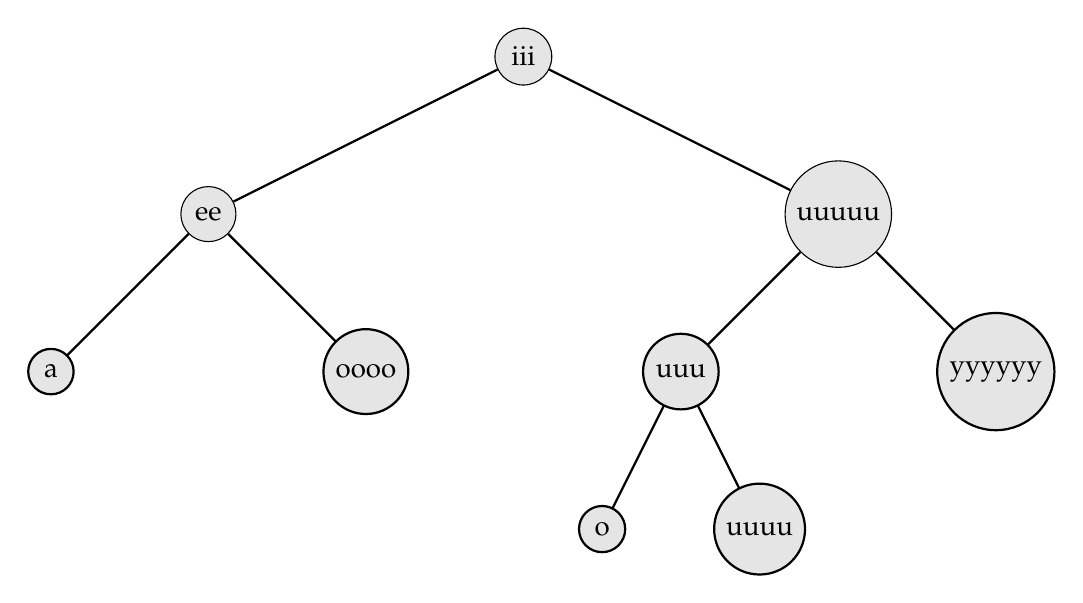
\begin{tikzpicture}[
      sibling distance=70mm,
      level distance=20mm,
      every node/.style={draw, fill=gray!20, circle},
      edge from parent/.style={draw, thick},
      level 1/.style={sibling distance=80mm},
      level 2/.style={sibling distance=40mm},
      level 3/.style={sibling distance=20mm}
    ]
      \node {iii}
        child { node {ee}
            child { node {a} }
            child { node {oooo} }
        }
        child { node {uuuuu}
            child { node {uuu}
            child { node {o} }
            child { node {uuuu} }
        }
            child { node {yyyyyy} }
        };
  \end{tikzpicture}
\end{center}

\begin{lstlisting}[style=Cstyle]
#include <stdio.h>

// Voici la fonction main.
int main() {
    printf("Hello, World!\n");
    return 0;
}
\end{lstlisting}

\end{document}
